% SPDX-License-Identifier: CC-BY-4.0
% Copyright (c) 2026 Jonathan Yantis. Results-focused research draft; not submitted.
\documentclass[10pt,letterpaper]{article}
\usepackage[margin=0.70in]{geometry}
\usepackage[T1]{fontenc}
\usepackage{mathptmx,amsmath,amssymb,booktabs,array,ragged2e,xcolor,microtype,xurl,hyperref,fancyhdr,tikz,pgfplots}
\usetikzlibrary{arrows.meta,positioning}\pgfplotsset{compat=1.18}
\definecolor{studyblue}{RGB}{32,75,103}\definecolor{studyorange}{RGB}{178,87,28}
\hypersetup{colorlinks=true,urlcolor=studyblue,citecolor=studyblue,linkcolor=black,pdfauthor={Jonathan Yantis},pdftitle={Precision Bluetooth Timing on ESP32-S3: Causal Clock Discipline and Hardware Event Capture}}
\setlength{\parindent}{1em}\setlength{\parskip}{3pt}\setlength{\headheight}{14pt}\setlength{\emergencystretch}{2em}
\widowpenalty=10000\clubpenalty=10000
\pagestyle{fancy}\fancyhf{}\fancyhead[L]{\small Precision Bluetooth Timing on ESP32-S3}\fancyhead[R]{\small Results-focused draft, 22 October 2026}\fancyfoot[C]{\small\thepage}
\newcommand{\ns}{\,\mathrm{ns}}\newcommand{\us}{\,\mu\mathrm{s}}\newcommand{\code}[1]{\texttt{#1}}\newcolumntype{L}[1]{>{\RaggedRight\arraybackslash}p{#1}}\renewcommand{\arraystretch}{1.15}
\newcommand{\FineTrace}{(0.95144037500,-114) (1.95144093750,-10) (2.95144143750,-257) (3.95144200000,-204) (4.95144250000,-202) (5.95144306250,-263) (6.95144356250,-187) (7.95144406250,-192) (8.95144462500,-242) (9.95144512500,-218) (10.95144575000,-32) (11.95144625000,-89) (12.95144681250,-140) (13.95144731250,-74) (14.95144787500,-144) (15.95144837500,-138) (16.95144893750,-40) (17.95144943750,-106) (18.95145000000,-75) (19.95145050000,-198) (20.95145106250,-284) (21.95145162500,-94) (22.95145212500,22) (23.95145268750,-239) (24.95145318750,-24) (25.95145368750,-186) (26.95145425000,-166) (27.95145481250,-106) (28.95145531250,-200) (29.95145587500,-29) (30.95145637500,-158) (31.95145693750,-41) (32.95145743750,-193) (33.95145800000,-92) (34.95145856250,98) (35.95145906250,-19) (36.95145962500,-48) (37.95146012500,-239) (38.95146062500,-174) (39.95146118750,-180) (40.95146168750,-224) (41.95146225000,-235) (42.95146275000,-187) (43.95146331250,-168) (44.95146381250,-275) (45.95146431250,-259) (46.95146487500,-225) (47.95146543750,-40) (48.95146593750,-143) (49.95146650000,-97) (50.95146706250,19) (51.95146756250,-7) (52.95146812500,90) (53.95146862500,-38) (54.95146918750,-53) (55.95146968750,-78) (56.95147018750,-237) (57.95147075000,-180) (58.95147125000,-195) (59.95147175000,-150) (60.95147231250,-96) (61.95147281250,-200) (62.95147331250,-226) (63.95147387500,-310) (64.95147437500,-264) (65.95147493750,-176) (66.95147543750,-256) (67.95147600000,-206) (68.95147650000,-19) (69.95147706250,-199) (70.95147762500,-131) (71.95147812500,-224) (72.95147868750,-88) (73.95147918750,-239) (74.95147975000,-97) (75.95148025000,-87) (76.95148081250,11) (77.95148131250,-79) (78.95148187500,-95) (79.95148237500,-256) (80.95148293750,-224) (81.95148343750,-189) (82.95148400000,-65) (83.95148450000,-97) (84.95148506250,-115) (85.95148556250,-110) (86.95148612500,-256) (87.95148662500,-98) (88.95148712500,-22) (89.95148768750,-67) (90.95148818750,8) (91.95148875000,-23) (92.95148931250,-213) (93.95148981250,-121) (94.95149037500,-18) (95.95149087500,-68) (96.95149143750,-39) (97.95149193750,-123) (98.95149250000,-75) (99.95149300000,-102) (100.95149356250,-222) (101.95149406250,-109) (102.95149456250,-130) (103.95149512500,-77) (104.95149568750,-233) (105.95149618750,-84) (106.95149668750,-84) (107.95149725000,-198) (108.95149775000,-165) (109.95149831250,-88) (110.95149881250,-134) (111.95149937500,-166) (112.95149987500,-186) (113.95150043750,-198) (114.95150093750,-103) (115.95150150000,-153) (116.95150200000,-119) (117.95150250000,-123) (118.95150306250,-30) (119.95150356250,-107) (120.95150412500,-100) (121.95150468750,-144) (122.95150518750,-15) (123.95150575000,-199) (124.95150625000,-250) (125.95150675000,-147) (126.95150731250,-109) (127.95150781250,-57) (128.95150837500,-27) (129.95150887500,-149) (130.95150943750,-73) (131.95150993750,-181) (132.95151050000,-212) (133.95151100000,-41) (134.95151150000,-213) (135.95151206250,-71) (136.95151256250,-124) (137.95151312500,-168) (138.95151362500,-109) (139.95151418750,-74) (140.95151468750,-161) (141.95151525000,-1591) (142.95151575000,-354) (143.95151625000,-161) (144.95151681250,-115) (145.95151731250,-163) (146.95151787500,-232) (147.95151837500,-154) (148.95151893750,-97) (149.95151950000,5) (150.95152000000,-25) (151.95152050000,-136) (152.95152106250,-147) (153.95152156250,-54) (154.95152212500,-76) (155.95152262500,-271) (156.95152312500,-175) (157.95152368750,-225) (158.95152418750,-195) (159.95152475000,-62) (160.95152525000,40) (161.95152581250,55) (162.95152631250,17) (163.95152681250,-87) (164.95152737500,-62) (165.95152787500,-251) (166.95152843750,-160) (167.95152893750,-119) (168.95152950000,-33) (169.95153000000,-103) (170.95153050000,-90) (171.95153106250,-20) (172.95153156250,-186) (173.95153212500,-192) (174.95153262500,20) (175.95153318750,20) (176.95153368750,-108) (177.95153418750,-42) (178.95153468750,-134) (179.95153525000,-1174) (180.95153581250,-123) (181.95153631250,-101) (182.95153687500,-170) (183.95153737500,-222) (184.95153787500,-94) (185.95153843750,-13) (186.95153900000,-12) (187.95153950000,-90) (188.95154000000,-118) (189.95154056250,-75) (190.95154106250,-173) (191.95154162500,-197) (192.95154212500,-88) (193.95154268750,-48) (194.95154318750,-196) (195.95154368750,-137) (196.95154425000,-215) (197.95154475000,58) (198.95154525000,-78) (199.95154581250,-73) (200.95154631250,-177) (201.95154687500,-77) (202.95154737500,-84) (203.95154793750,-84) (204.95154843750,-53) (205.95154893750,-107) (206.95154943750,-283) (207.95155000000,-243) (208.95155050000,-279) (209.95155100000,-48) (210.95155156250,-14) (211.95155212500,81) (212.95155262500,-118) (213.95155318750,-19) (214.95155368750,-158) (215.95155418750,-195) (216.95155475000,-163) (217.95155525000,-197) (218.95155575000,-283) (219.95155631250,-213) (220.95155687500,-108) (221.95155737500,59) (222.95155787500,-54) (223.95155843750,-3) (224.95155893750,-58) (225.95155943750,-133) (226.95156000000,-65) (227.95156050000,-37) (228.95156106250,92) (229.95156156250,-32) (230.95156212500,-66) (231.95156262500,-104) (232.95156312500,24) (233.95156362500,-66) (234.95156418750,-108) (235.95156468750,-72) (236.95156525000,-28) (237.95156575000,4) (238.95156631250,-87) (239.95156681250,-96) (240.95156731250,-186) (241.95156781250,-160) (242.95156837500,19) (243.95156893750,-4) (244.95156943750,-130) (245.95157000000,79) (246.95157050000,150) (247.95157100000,-171) (248.95157156250,42) (249.95157200000,-202) (250.95157256250,-139) (251.95157306250,-75) (252.95157356250,29) (253.95157412500,-55) (254.95157468750,83) (255.95157518750,-127) (256.95157568750,-37) (257.95157618750,-111) (258.95157675000,-182) (259.95157725000,-34) (260.95157781250,-66) (261.95157831250,-136) (262.95157881250,-172) (263.95157931250,-90) (264.95157987500,-76) (265.95158043750,-179) (266.95158093750,-94) (267.95158143750,-122) (268.95158200000,-63) (269.95158250000,-21) (270.95158300000,-184) (271.95158356250,-143) (272.95158406250,-127) (273.95158456250,-66) (274.95158512500,-39) (275.95158562500,-128) (276.95158618750,33) (277.95158668750,-357) (278.95158718750,-198) (279.95158775000,-142) (280.95158825000,52) (281.95158875000,-87) (282.95158931250,-179) (283.95158981250,25) (284.95159031250,-25) (285.95159087500,-202) (286.95159137500,-56) (287.95159193750,-190) (288.95159243750,-148) (289.95159293750,-22) (290.95159350000,-96) (291.95159400000,-158) (292.95159456250,-139) (293.95159506250,-110) (294.95159556250,-48) (295.95159612500,-32) (296.95159662500,-103) (297.95159718750,-101) (298.95159775000,-55) (299.95159825000,47) (300.95159875000,-143) (301.95159925000,-159) (302.95159981250,-129) (303.95160031250,46) (304.95160081250,-195) (305.95160137500,-22) (306.95160193750,-86) (307.95160243750,-79) (308.95160300000,-2) (309.95160350000,-179) (310.95160400000,-106) (311.95160456250,-138) (312.95160506250,-35) (313.95160562500,33) (314.95160612500,-214) (315.95160668750,-114) (316.95160718750,-150) (317.95160775000,nan) (318.95160825000,-222) (319.95160881250,-31) (320.95160931250,-80) (321.95160987500,-145) (322.95161043750,nan) (323.95161100000,-68) (324.95161150000,-18) (325.95161200000,-228) (326.95161256250,-129) (327.95161306250,-45) (328.95161362500,12) (329.95161418750,-59) (330.95161468750,-39) (331.95161525000,-87) (332.95161575000,-112) (333.95161631250,-246) (334.95161687500,-151) (335.95161743750,-49) (336.95161793750,-128) (337.95161850000,46) (338.95161906250,26) (339.95161956250,-29) (340.95162012500,-89) (341.95162068750,-58) (342.95162118750,-56) (343.95162168750,-108) (344.95162225000,-86) (345.95162281250,-109) (346.95162337500,-72) (347.95162387500,-122) (348.95162443750,-136) (349.95162500000,-81) (350.95162556250,190) (351.95162606250,-157) (352.95162662500,17) (353.95162718750,19) (354.95162768750,-95) (355.95162825000,-41) (356.95162881250,2) (357.95162931250,-109) (358.95162987500,-88) (359.95163037500,-223) (360.95163093750,-220) (361.95163150000,-69) (362.95163200000,-145) (363.95163256250,-178) (364.95163312500,-121) (365.95163368750,-135) (366.95163425000,90) (367.95163475000,-33) (368.95163531250,20) (369.95163581250,-229) (370.95163637500,-104) (371.95163687500,-132) (372.95163743750,-123) (373.95163800000,-79) (374.95163850000,-71) (375.95163906250,-82) (376.95163962500,-175) (377.95164018750,-161) (378.95164075000,-133) (379.95164131250,-100) (380.95164187500,-69) (381.95164243750,-99) (382.95164293750,-206) (383.95164350000,-58) (384.95164400000,-31) (385.95164456250,62) (386.95164512500,-29) (387.95164568750,-66) (388.95164625000,83) (389.95164675000,-169) (390.95164731250,-97) (391.95164787500,-107) (392.95164837500,-84) (393.95164900000,-157) (394.95164950000,-56) (395.95165006250,-101) (396.95165062500,-58) (397.95165112500,-37) (398.95165168750,-13) (399.95165225000,53) (400.95165281250,21) (401.95165331250,-261) (402.95165393750,-88) (403.95165443750,-273) (404.95165500000,-269) (405.95165556250,-102) (406.95165606250,-6) (407.95165662500,-147) (408.95165712500,-184) (409.95165768750,-98) (410.95165825000,-150) (411.95165881250,-157) (412.95165937500,-175) (413.95165993750,-38) (414.95166050000,36) (415.95166100000,-104) (416.95166156250,-147) (417.95166212500,15) (418.95166275000,23) (419.95166325000,-54) (420.95166381250,-214) (421.95166437500,-1312) (422.95166493750,-54) (423.95166550000,-70) (424.95166606250,-43) (425.95166656250,-1239) (426.95166712500,-46) (427.95166768750,-4) (428.95166825000,3) (429.95166875000,-95) (430.95166931250,-55) (431.95166993750,-53) (432.95167043750,-118) (433.95167100000,149) (434.95167156250,76) (435.95167212500,-110) (436.95167268750,-54) (437.95167318750,10) (438.95167375000,-133) (439.95167431250,-159) (440.95167487500,0) (441.95167543750,-10) (442.95167600000,-176) (443.95167650000,-266) (444.95167706250,-113) (445.95167762500,-59) (446.95167818750,91) (447.95167875000,-9) (448.95167931250,-100) (449.95167987500,59) (450.95168043750,89) (451.95168100000,51) (452.95168150000,111) (453.95168206250,-48) (454.95168262500,-98) (455.95168318750,-61) (456.95168375000,-66) (457.95168431250,-70) (458.95168481250,-62) (459.95168543750,-67) (460.95168593750,-160) (461.95168650000,-235) (462.95168706250,-215) (463.95168762500,-171) (464.95168818750,-14) (465.95168875000,-53) (466.95168931250,-104) (467.95168987500,92) (468.95169043750,-177) (469.95169100000,-12) (470.95169156250,-82) (471.95169206250,-142) (472.95169268750,-35) (473.95169318750,10) (474.95169375000,-110) (475.95169431250,-23) (476.95169487500,-47) (477.95169543750,-98) (478.95169593750,28) (479.95169650000,-81) (480.95169706250,12) (481.95169762500,-150) (482.95169818750,-94) (483.95169875000,-88) (484.95169931250,-65) (485.95169987500,-29) (486.95170043750,38) (487.95170093750,-72) (488.95170150000,184) (489.95170206250,5) (490.95170262500,-160) (491.95170318750,-11) (492.95170375000,-19) (493.95170431250,-18) (494.95170487500,-155) (495.95170537500,-244) (496.95170593750,-163) (497.95170650000,-36) (498.95170706250,-142) (499.95170762500,-74) (500.95170818750,-89) (501.95170875000,-140) (502.95170931250,-20) (503.95170987500,-89) (504.95171043750,-23) (505.95171093750,-197) (506.95171150000,-207) (507.95171206250,-85) (508.95171262500,-192) (509.95171318750,-140) (510.95171375000,-161) (511.95171431250,-76) (512.95171487500,-122) (513.95171543750,-135) (514.95171600000,-169) (515.95171656250,-142) (516.95171706250,-151) (517.95171762500,-153) (518.95171818750,-181) (519.95171875000,-148) (520.95171931250,-212) (521.95171987500,-128) (522.95172043750,-80) (523.95172100000,-128) (524.95172156250,83) (525.95172212500,-124) (526.95172262500,-289) (527.95172325000,-170) (528.95172381250,-132) (529.95172431250,-76) (530.95172487500,-130) (531.95172543750,-92) (532.95172600000,-112) (533.95172656250,-168) (534.95172712500,-7) (535.95172768750,-65) (536.95172825000,-173) (537.95172881250,-212) (538.95172937500,-75) (539.95172993750,-166) (540.95173050000,-136) (541.95173106250,-106) (542.95173162500,-105) (543.95173218750,-140) (544.95173275000,-112) (545.95173331250,-98) (546.95173381250,-95) (547.95173437500,-137) (548.95173493750,-71) (549.95173550000,-211) (550.95173606250,-199) (551.95173662500,-126) (552.95173718750,-81) (553.95173775000,-121) (554.95173831250,-108) (555.95173887500,-186) (556.95173943750,-23) (557.95174006250,134) (558.95174056250,63) (559.95174112500,-37) (560.95174175000,-32) (561.95174231250,27) (562.95174281250,-92) (563.95174337500,-140) (564.95174393750,-175) (565.95174450000,-29) (566.95174506250,-37) (567.95174562500,-85) (568.95174618750,-125) (569.95174675000,-89) (570.95174731250,-61) (571.95174787500,-152) (572.95174850000,35) (573.95174906250,-42) (574.95174956250,-192) (575.95175012500,-50) (576.95175068750,-18) (577.95175125000,-41) (578.95175181250,-161) (579.95175237500,-110) (580.95175293750,-113) (581.95175350000,-54) (582.95175406250,-183) (583.95175462500,-67) (584.95175518750,-97) (585.95175575000,-186) (586.95175631250,-40) (587.95175687500,-36) (588.95175743750,-65) (589.95175800000,7) (590.95175856250,-26) (591.95175912500,-33) (592.95175968750,-33) (593.95176025000,-77) (594.95176081250,-190) (595.95176137500,-104) (596.95176193750,-67) (597.95176250000,-70) (598.95176306250,-122) (599.95176362500,-159) (600.95176418750,4) (601.95176475000,-61) (602.95176531250,-138) (603.95176587500,-97) (604.95176643750,-179) (605.95176700000,-13) (606.95176756250,-80) (607.95176812500,-157) (608.95176868750,-23) (609.95176925000,-197) (610.95176987500,-162) (611.95177043750,-116) (612.95177100000,-58) (613.95177156250,-181) (614.95177212500,-169) (615.95177268750,-131) (616.95177325000,-8) (617.95177381250,59) (618.95177443750,-8) (619.95177500000,-29) (620.95177550000,-161) (621.95177606250,-58) (622.95177662500,8) (623.95177718750,-107) (624.95177775000,-126) (625.95177831250,-49) (626.95177887500,-111) (627.95177943750,-44) (628.95178000000,-142) (629.95178056250,-208) (630.95178112500,-171) (631.95178168750,-299) (632.95178225000,-154) (633.95178287500,-96) (634.95178343750,-114) (635.95178400000,nan) (636.95178456250,-36) (637.95178512500,-13) (638.95178568750,-188) (639.95178625000,-62) (640.95178681250,-36) (641.95178737500,-84) (642.95178793750,-41) (643.95178856250,-90) (644.95178912500,-45) (645.95178962500,-107) (646.95179018750,-143) (647.95179081250,-129) (648.95179137500,-165) (649.95179193750,-111) (650.95179250000,-74) (651.95179306250,-122) (652.95179362500,-179) (653.95179418750,-164) (654.95179475000,-56) (655.95179531250,-168) (656.95179587500,-83) (657.95179643750,-79) (658.95179706250,-94) (659.95179756250,1)}
\newcommand{\InvalidTrace}{(317.95160775000,0) (322.95161043750,0) (635.95178400000,0)}
\newcommand{\FineEcdf}{(1,0.0015220700) (1,0.0030441400) (2,0.0045662100) (2,0.0060882801) (3,0.0076103501) (3,0.0091324201) (4,0.0106544901) (4,0.0121765601) (4,0.0136986301) (4,0.0152207002) (5,0.0167427702) (5,0.0182648402) (6,0.0197869102) (7,0.0213089802) (7,0.0228310502) (7,0.0243531202) (8,0.0258751903) (8,0.0273972603) (8,0.0289193303) (8,0.0304414003) (9,0.0319634703) (10,0.0334855403) (10,0.0350076104) (10,0.0365296804) (10,0.0380517504) (11,0.0395738204) (11,0.0410958904) (12,0.0426179604) (12,0.0441400304) (12,0.0456621005) (12,0.0471841705) (13,0.0487062405) (13,0.0502283105) (13,0.0517503805) (13,0.0532724505) (14,0.0547945205) (14,0.0563165906) (15,0.0578386606) (15,0.0593607306) (17,0.0608828006) (17,0.0624048706) (18,0.0639269406) (18,0.0654490107) (18,0.0669710807) (18,0.0684931507) (19,0.0700152207) (19,0.0715372907) (19,0.0730593607) (19,0.0745814307) (19,0.0761035008) (19,0.0776255708) (19,0.0791476408) (20,0.0806697108) (20,0.0821917808) (20,0.0837138508) (20,0.0852359209) (20,0.0867579909) (21,0.0882800609) (21,0.0898021309) (22,0.0913242009) (22,0.0928462709) (22,0.0943683409) (22,0.0958904110) (23,0.0974124810) (23,0.0989345510) (23,0.1004566210) (23,0.1019786910) (23,0.1035007610) (23,0.1050228311) (24,0.1065449011) (24,0.1080669711) (25,0.1095890411) (25,0.1111111111) (25,0.1126331811) (26,0.1141552511) (26,0.1156773212) (27,0.1171993912) (27,0.1187214612) (28,0.1202435312) (28,0.1217656012) (29,0.1232876712) (29,0.1248097412) (29,0.1263318113) (29,0.1278538813) (29,0.1293759513) (29,0.1308980213) (29,0.1324200913) (30,0.1339421613) (31,0.1354642314) (31,0.1369863014) (32,0.1385083714) (32,0.1400304414) (32,0.1415525114) (32,0.1430745814) (33,0.1445966514) (33,0.1461187215) (33,0.1476407915) (33,0.1491628615) (33,0.1506849315) (33,0.1522070015) (34,0.1537290715) (35,0.1552511416) (35,0.1567732116) (35,0.1582952816) (36,0.1598173516) (36,0.1613394216) (36,0.1628614916) (36,0.1643835616) (36,0.1659056317) (37,0.1674277017) (37,0.1689497717) (37,0.1704718417) (37,0.1719939117) (37,0.1735159817) (38,0.1750380518) (38,0.1765601218) (38,0.1780821918) (39,0.1796042618) (39,0.1811263318) (39,0.1826484018) (40,0.1841704718) (40,0.1856925419) (40,0.1872146119) (40,0.1887366819) (41,0.1902587519) (41,0.1917808219) (41,0.1933028919) (41,0.1948249619) (41,0.1963470320) (42,0.1978691020) (42,0.1993911720) (42,0.2009132420) (43,0.2024353120) (44,0.2039573820) (45,0.2054794521) (45,0.2070015221) (46,0.2085235921) (46,0.2100456621) (46,0.2115677321) (47,0.2130898021) (47,0.2146118721) (48,0.2161339422) (48,0.2176560122) (48,0.2191780822) (48,0.2207001522) (48,0.2222222222) (49,0.2237442922) (49,0.2252663623) (50,0.2267884323) (51,0.2283105023) (52,0.2298325723) (53,0.2313546423) (53,0.2328767123) (53,0.2343987823) (53,0.2359208524) (53,0.2374429224) (54,0.2389649924) (54,0.2404870624) (54,0.2420091324) (54,0.2435312024) (54,0.2450532725) (54,0.2465753425) (55,0.2480974125) (55,0.2496194825) (55,0.2511415525) (55,0.2526636225) (56,0.2541856925) (56,0.2557077626) (56,0.2572298326) (56,0.2587519026) (57,0.2602739726) (58,0.2617960426) (58,0.2633181126) (58,0.2648401826) (58,0.2663622527) (58,0.2678843227) (58,0.2694063927) (58,0.2709284627) (59,0.2724505327) (59,0.2739726027) (59,0.2754946728) (59,0.2770167428) (59,0.2785388128) (61,0.2800608828) (61,0.2815829528) (61,0.2831050228) (62,0.2846270928) (62,0.2861491629) (62,0.2876712329) (62,0.2891933029) (62,0.2907153729) (63,0.2922374429) (63,0.2937595129) (65,0.2952815830) (65,0.2968036530) (65,0.2983257230) (65,0.2998477930) (65,0.3013698630) (66,0.3028919330) (66,0.3044140030) (66,0.3059360731) (66,0.3074581431) (66,0.3089802131) (66,0.3105022831) (67,0.3120243531) (67,0.3135464231) (67,0.3150684932) (67,0.3165905632) (68,0.3181126332) (68,0.3196347032) (69,0.3211567732) (69,0.3226788432) (70,0.3242009132) (70,0.3257229833) (70,0.3272450533) (71,0.3287671233) (71,0.3302891933) (71,0.3318112633) (72,0.3333333333) (72,0.3348554033) (72,0.3363774734) (73,0.3378995434) (73,0.3394216134) (74,0.3409436834) (74,0.3424657534) (74,0.3439878234) (74,0.3455098935) (75,0.3470319635) (75,0.3485540335) (75,0.3500761035) (75,0.3515981735) (75,0.3531202435) (76,0.3546423135) (76,0.3561643836) (76,0.3576864536) (76,0.3592085236) (76,0.3607305936) (77,0.3622526636) (77,0.3637747336) (77,0.3652968037) (78,0.3668188737) (78,0.3683409437) (79,0.3698630137) (79,0.3713850837) (79,0.3729071537) (79,0.3744292237) (79,0.3759512938) (80,0.3774733638) (80,0.3789954338) (80,0.3805175038) (81,0.3820395738) (81,0.3835616438) (81,0.3850837139) (81,0.3866057839) (82,0.3881278539) (82,0.3896499239) (83,0.3911719939) (83,0.3926940639) (83,0.3942161339) (83,0.3957382040) (84,0.3972602740) (84,0.3987823440) (84,0.4003044140) (84,0.4018264840) (84,0.4033485540) (84,0.4048706240) (85,0.4063926941) (85,0.4079147641) (86,0.4094368341) (86,0.4109589041) (87,0.4124809741) (87,0.4140030441) (87,0.4155251142) (87,0.4170471842) (87,0.4185692542) (88,0.4200913242) (88,0.4216133942) (88,0.4231354642) (88,0.4246575342) (88,0.4261796043) (88,0.4277016743) (89,0.4292237443) (89,0.4307458143) (89,0.4322678843) (89,0.4337899543) (89,0.4353120244) (89,0.4368340944) (90,0.4383561644) (90,0.4398782344) (90,0.4414003044) (90,0.4429223744) (90,0.4444444444) (90,0.4459665145) (91,0.4474885845) (92,0.4490106545) (92,0.4505327245) (92,0.4520547945) (92,0.4535768645) (92,0.4550989346) (94,0.4566210046) (94,0.4581430746) (94,0.4596651446) (94,0.4611872146) (94,0.4627092846) (95,0.4642313546) (95,0.4657534247) (95,0.4672754947) (95,0.4687975647) (96,0.4703196347) (96,0.4718417047) (96,0.4733637747) (96,0.4748858447) (97,0.4764079148) (97,0.4779299848) (97,0.4794520548) (97,0.4809741248) (97,0.4824961948) (97,0.4840182648) (97,0.4855403349) (98,0.4870624049) (98,0.4885844749) (98,0.4901065449) (98,0.4916286149) (98,0.4931506849) (98,0.4946727549) (99,0.4961948250) (100,0.4977168950) (100,0.4992389650) (100,0.5007610350) (101,0.5022831050) (101,0.5038051750) (101,0.5053272451) (102,0.5068493151) (102,0.5083713851) (103,0.5098934551) (103,0.5114155251) (103,0.5129375951) (104,0.5144596651) (104,0.5159817352) (104,0.5175038052) (104,0.5190258752) (104,0.5205479452) (105,0.5220700152) (106,0.5235920852) (106,0.5251141553) (106,0.5266362253) (106,0.5281582953) (107,0.5296803653) (107,0.5312024353) (107,0.5327245053) (107,0.5342465753) (107,0.5357686454) (108,0.5372907154) (108,0.5388127854) (108,0.5403348554) (108,0.5418569254) (108,0.5433789954) (109,0.5449010654) (109,0.5464231355) (109,0.5479452055) (109,0.5494672755) (109,0.5509893455) (110,0.5525114155) (110,0.5540334855) (110,0.5555555556) (110,0.5570776256) (110,0.5585996956) (111,0.5601217656) (111,0.5616438356) (111,0.5631659056) (111,0.5646879756) (112,0.5662100457) (112,0.5677321157) (112,0.5692541857) (113,0.5707762557) (113,0.5722983257) (114,0.5738203957) (114,0.5753424658) (114,0.5768645358) (115,0.5783866058) (115,0.5799086758) (116,0.5814307458) (118,0.5829528158) (118,0.5844748858) (118,0.5859969559) (119,0.5875190259) (119,0.5890410959) (121,0.5905631659) (121,0.5920852359) (121,0.5936073059) (122,0.5951293760) (122,0.5966514460) (122,0.5981735160) (122,0.5996955860) (122,0.6012176560) (123,0.6027397260) (123,0.6042617960) (123,0.6057838661) (123,0.6073059361) (124,0.6088280061) (124,0.6103500761) (125,0.6118721461) (126,0.6133942161) (126,0.6149162861) (127,0.6164383562) (127,0.6179604262) (128,0.6194824962) (128,0.6210045662) (128,0.6225266362) (128,0.6240487062) (129,0.6255707763) (129,0.6270928463) (129,0.6286149163) (130,0.6301369863) (130,0.6316590563) (130,0.6331811263) (131,0.6347031963) (131,0.6362252664) (132,0.6377473364) (132,0.6392694064) (133,0.6407914764) (133,0.6423135464) (133,0.6438356164) (134,0.6453576865) (134,0.6468797565) (134,0.6484018265) (135,0.6499238965) (135,0.6514459665) (136,0.6529680365) (136,0.6544901065) (136,0.6560121766) (136,0.6575342466) (137,0.6590563166) (137,0.6605783866) (138,0.6621004566) (138,0.6636225266) (138,0.6651445967) (139,0.6666666667) (139,0.6681887367) (140,0.6697108067) (140,0.6712328767) (140,0.6727549467) (140,0.6742770167) (140,0.6757990868) (142,0.6773211568) (142,0.6788432268) (142,0.6803652968) (142,0.6818873668) (142,0.6834094368) (143,0.6849315068) (143,0.6864535769) (143,0.6879756469) (143,0.6894977169) (144,0.6910197869) (144,0.6925418569) (145,0.6940639269) (145,0.6955859970) (147,0.6971080670) (147,0.6986301370) (147,0.7001522070) (147,0.7016742770) (148,0.7031963470) (148,0.7047184170) (149,0.7062404871) (149,0.7077625571) (150,0.7092846271) (150,0.7108066971) (150,0.7123287671) (150,0.7138508371) (150,0.7153729072) (151,0.7168949772) (151,0.7184170472) (152,0.7199391172) (153,0.7214611872) (153,0.7229832572) (154,0.7245053272) (154,0.7260273973) (155,0.7275494673) (157,0.7290715373) (157,0.7305936073) (157,0.7321156773) (157,0.7336377473) (158,0.7351598174) (158,0.7366818874) (158,0.7382039574) (159,0.7397260274) (159,0.7412480974) (159,0.7427701674) (160,0.7442922374) (160,0.7458143075) (160,0.7473363775) (160,0.7488584475) (161,0.7503805175) (161,0.7519025875) (161,0.7534246575) (161,0.7549467275) (161,0.7564687976) (161,0.7579908676) (162,0.7595129376) (163,0.7610350076) (163,0.7625570776) (163,0.7640791476) (164,0.7656012177) (165,0.7671232877) (165,0.7686453577) (166,0.7701674277) (166,0.7716894977) (166,0.7732115677) (168,0.7747336377) (168,0.7762557078) (168,0.7777777778) (168,0.7792998478) (169,0.7808219178) (169,0.7823439878) (169,0.7838660578) (170,0.7853881279) (170,0.7869101979) (171,0.7884322679) (171,0.7899543379) (171,0.7914764079) (172,0.7929984779) (173,0.7945205479) (173,0.7960426180) (174,0.7975646880) (175,0.7990867580) (175,0.8006088280) (175,0.8021308980) (175,0.8036529680) (176,0.8051750381) (176,0.8066971081) (177,0.8082191781) (177,0.8097412481) (178,0.8112633181) (179,0.8127853881) (179,0.8143074581) (179,0.8158295282) (179,0.8173515982) (179,0.8188736682) (180,0.8203957382) (180,0.8219178082) (181,0.8234398782) (181,0.8249619482) (181,0.8264840183) (182,0.8280060883) (183,0.8295281583) (184,0.8310502283) (184,0.8325722983) (184,0.8340943683) (186,0.8356164384) (186,0.8371385084) (186,0.8386605784) (186,0.8401826484) (186,0.8417047184) (186,0.8432267884) (187,0.8447488584) (187,0.8462709285) (188,0.8477929985) (189,0.8493150685) (190,0.8508371385) (190,0.8523592085) (190,0.8538812785) (192,0.8554033486) (192,0.8569254186) (192,0.8584474886) (192,0.8599695586) (193,0.8614916286) (195,0.8630136986) (195,0.8645357686) (195,0.8660578387) (195,0.8675799087) (196,0.8691019787) (197,0.8706240487) (197,0.8721461187) (197,0.8736681887) (197,0.8751902588) (198,0.8767123288) (198,0.8782343988) (198,0.8797564688) (198,0.8812785388) (199,0.8828006088) (199,0.8843226788) (199,0.8858447489) (200,0.8873668189) (200,0.8888888889) (202,0.8904109589) (202,0.8919330289) (202,0.8934550989) (204,0.8949771689) (206,0.8964992390) (206,0.8980213090) (207,0.8995433790) (208,0.9010654490) (211,0.9025875190) (212,0.9041095890) (212,0.9056316591) (212,0.9071537291) (213,0.9086757991) (213,0.9101978691) (213,0.9117199391) (214,0.9132420091) (214,0.9147640791) (215,0.9162861492) (215,0.9178082192) (218,0.9193302892) (220,0.9208523592) (222,0.9223744292) (222,0.9238964992) (222,0.9254185693) (223,0.9269406393) (224,0.9284627093) (224,0.9299847793) (224,0.9315068493) (225,0.9330289193) (225,0.9345509893) (226,0.9360730594) (228,0.9375951294) (229,0.9391171994) (232,0.9406392694) (233,0.9421613394) (235,0.9436834094) (235,0.9452054795) (237,0.9467275495) (239,0.9482496195) (239,0.9497716895) (239,0.9512937595) (242,0.9528158295) (243,0.9543378995) (244,0.9558599696) (246,0.9573820396) (250,0.9589041096) (251,0.9604261796) (256,0.9619482496) (256,0.9634703196) (256,0.9649923896) (257,0.9665144597) (259,0.9680365297) (261,0.9695585997) (263,0.9710806697) (264,0.9726027397) (266,0.9741248097) (269,0.9756468798) (271,0.9771689498) (273,0.9786910198) (275,0.9802130898) (279,0.9817351598) (283,0.9832572298) (283,0.9847792998) (284,0.9863013699) (289,0.9878234399) (299,0.9893455099) (310,0.9908675799) (354,0.9923896499) (357,0.9939117199) (1174,0.9954337900) (1239,0.9969558600) (1312,0.9984779300) (1591,1.0000000000)}
\newcommand{\SubsetEcdf}{(10,0.0208333333) (19,0.0416666667) (22,0.0625000000) (24,0.0833333333) (29,0.1041666667) (32,0.1250000000) (40,0.1458333333) (40,0.1666666667) (41,0.1875000000) (48,0.2083333333) (74,0.2291666667) (75,0.2500000000) (89,0.2708333333) (92,0.2916666667) (94,0.3125000000) (98,0.3333333333) (106,0.3541666667) (106,0.3750000000) (114,0.3958333333) (138,0.4166666667) (140,0.4375000000) (144,0.4583333333) (158,0.4791666667) (166,0.5000000000) (168,0.5208333333) (174,0.5416666667) (180,0.5625000000) (186,0.5833333333) (187,0.6041666667) (187,0.6250000000) (192,0.6458333333) (193,0.6666666667) (198,0.6875000000) (200,0.7083333333) (202,0.7291666667) (204,0.7500000000) (218,0.7708333333) (224,0.7916666667) (225,0.8125000000) (235,0.8333333333) (239,0.8541666667) (239,0.8750000000) (242,0.8958333333) (257,0.9166666667) (259,0.9375000000) (263,0.9583333333) (275,0.9791666667) (284,1.0000000000)}
\newcommand{\FinalTableRow}{N31 51,016; fresh transfer48 &48&115.167&150.954&97.590&362\\}
\newcommand{\FinalResults}{A fresh second-board N31 transfer on the same total yielded 48 eligible of 64 records, with 16 reason-2 invalid, zero sequence gaps/duplicates and one terminal unread edge. Mean was $+115.167\ns$, RMS 150.954 ns, standard deviation 97.590 ns and maximum 362 ns over a 63.000031 s eligible span. The total was not mean-zero portable; the sub-100 ns target failed. No retuning or N31 TX packet-log proof is part of this separate short observation.}
\begin{document}
\title{\vspace{-1.5em}Precision Bluetooth Timing on ESP32-S3:\\Causal Clock Discipline and Hardware Event Capture}
\author{Jonathan Yantis\\\small Independent researcher}
\date{22 October 2026, measured-results follow-up\\\small Research draft; not submitted or peer reviewed}
\maketitle\vspace{-1em}
\begin{abstract}
An implemented ESP32-S3 receive-capture backend completed a fixed 660 s downstream relative-PPS experiment with 657 eligible observations, three invalid records, zero nominal missing opportunities and an observed post-window fence. The actual eligible mean was $-106.811\ns$, uncentered RMS 166.590 ns, standard deviation 127.842 ns and maximum absolute residual 1591 ns. Four retained excursions above 1 $\mu$s account for 39.302\% of the uncentered squared error. The result meets the finite collection-coverage objective but fails the sub-100 ns output target. A separate prespecified sparse comparison scored 62 of 64 held-out opportunities: empirical fine-marker RMS was 171.004 ns versus 259.324 ns for matched legacy descriptors. Near-50 ns internal causal clock-quality readings remain distinct from delivered downstream PPS error. The backend joins exact retained packets to RX-active falling edges on one continuing 80 MHz counter; its RF endpoint is unqualified and TX remains a programmed software estimate. The earlier final-profile short legacy check (48 eligible, 99.608 ns RMS) and incomplete legacy 660 s attempt retain separate populations and missingness. The new 660 s population subsequently selected a provisional 51,016 ns composite offset and cannot validate it. A fresh same-offset N31 transfer retained 48 eligible and 16 invalid records, with 150.954 ns RMS and $+115.167\ns$ mean, failing the output target. This report documents the measurements, fault repairs, reproducible accounting and concrete remaining work on TX capture, RX endpoint/delay, tails and fresh transfer validation.
\end{abstract}
\noindent\footnotesize Copyright \copyright\ 2026 Jonathan Yantis. Paper, figures and derived evidence: \href{https://creativecommons.org/licenses/by/4.0/}{CC BY 4.0}. Code and ordinary documentation: MIT.\normalsize

\section{Measured findings and scope}\label{sec:findings}
The main completed observation is a heterogeneous BLE path: an upstream Nordic source, an ESP32-S3 N30 receiver/estimated relay and a downstream Nordic T096 witness. The N30 has no GNSS. The witness evaluates its delivered BLE map at a locally captured physical PPS; it does not measure an N30 output pin. Its absolute PPS-to-UTC association is unavailable. Every accuracy-like value here is signed fractional-second, source-relative phase unless explicitly identified as an internal or counter-comparison metric.

Three findings govern interpretation. First, the new capture backend and repaired firmware sustained a complete finite 660 s exported record population; the previous collection ending had failed. Second, packet-associated marker capture improved a separate matched causal comparison, while its uncentered RMS still exceeded the target. Third, the complete delivered PPS result retained bias and four large tails. Neither finer timer units nor the internal fit score explains those tails away.

The publication/relay correction was frozen at 50,909 ns before the completed window. All eligible phase values, the three invalid records, the window boundary and terminal fence are retained in the selected supplement. No retrospective offset, channel correction, residual cut or tail removal changes the reported 166.590 ns RMS. Reusing this population afterward to choose 51,016 ns changes its role for the next profile, not its original measured result.

The earlier reviewed edition remains preserved in Git and its original receipt \cite{previous}. This revision reports implemented changes and completed observations; it does not pool different source paths, boots, estimators or reference conventions into one benchmark. The following pages begin with output coverage and tails, then show calibration, the implemented capture path, the controlled comparison and the remaining measured limitations.
\newpage

\section{The complete 660-second record}\label{sec:full}
\subsection{Coverage was recovered; the output target was not}
The prespecified interval uses the witness's nominal 16 MHz native counter, inclusive start and exclusive end separated by exactly 660 s in one local capture epoch. All 660 in-window records were exported: 657 eligible, three reason-2 invalid, zero sequence gaps and zero duplicates. A post-window sequence fence was observed. Nominal 1 Hz accounting is $660=657+3+0$ eligible, invalid and unrecorded opportunities; eligible coverage is 99.545\%. This is an opportunity model, not an independent physical count of all pulses.

Eligible edges span 659.000357 s. Mean is $-106.811\ns$, uncentered RMS 166.590 ns and standard deviation 127.842 ns. Absolute P50/P95/P99 are $100/239/310\ns$, with signed range $-1591$ to $190\ns$. The complete trace retains the eligible extremes and breaks at invalid rows; their stored numeric values are not scored.

\begin{figure}[ht]
\centering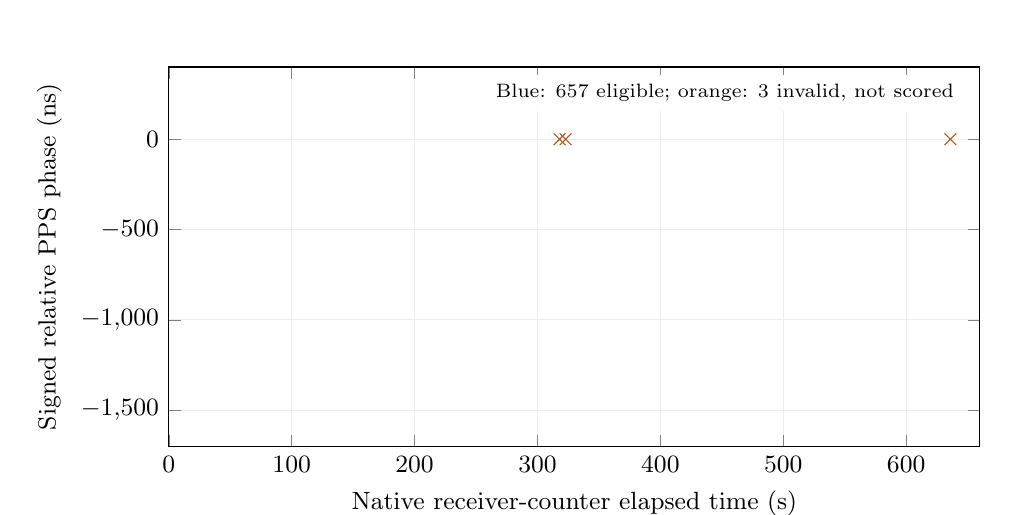
\begin{tikzpicture}
\begin{axis}[width=.98\linewidth,height=64mm,xmin=0,xmax=660,ymin=-1700,ymax=400,xlabel={Native receiver-counter elapsed time (s)},ylabel={Signed relative PPS phase (ns)},grid=major,grid style={gray!15},tick label style={font=\small},label style={font=\small},scaled y ticks=false,unbounded coords=jump]
\addplot[studyblue,thin,mark=none] coordinates {\FineTrace};
\addplot[studyorange,only marks,mark=x,mark size=3pt] coordinates {\InvalidTrace};
\node[anchor=north east,font=\scriptsize,fill=white] at (rel axis cs:.98,.98) {Blue: 657 eligible; orange: 3 invalid, not scored};
\end{axis}\end{tikzpicture}
\caption{All retained phase values on the full prespecified 660 s axis. No fitted validation offset or detrending is applied. Four eligible excursions exceed 1 $\mu$s. Invalid crosses show stored phase only; they do not improve the residual score.}
\end{figure}

\begin{table}[ht]\centering\small
\caption{The four largest eligible excursions, retained in every headline statistic. Relative times use the original fixed-window origin.}
\begin{tabular}{rrrr}\toprule
Elapsed s & Signed phase ns & Elapsed s & Signed phase ns\\\midrule
141.951515 &$-1591$&179.951535 &$-1174$\\
421.951664 &$-1312$&425.951667 &$-1239$\\\bottomrule
\end{tabular}\end{table}

These four records are 0.609\% of the eligible population and contribute 39.302\% of its uncentered squared error. Seventy-three of 657 eligible residuals exceed 200 ns in absolute value. This accounting describes the concentration of error; no trimmed score replaces the full result. The cause of the excursions is not isolated by this experiment.

Three unread terminal edges occurred \emph{after} the observed post-window fence and are not in-window missing records. Queue-drop and disabled-edge deltas were zero. The collection lasted 664.023 s after its native start, including fence/drain. Counter checks, transport accounting and empty polls are described with the method and supplement; a complete software export does not establish calibrated UTC or RF endpoint accuracy.
\newpage

\section{Calibration, short checks and historical coverage}\label{sec:calibration}
\subsection{Fine calibration was frozen before the completed window}
The fine-backend calibration run retained 51 records: the first 48 eligible plus three reason-2 invalid. It had no interior gaps and one terminal unread edge. With nominal programmed-to-advertised totals of 39,999 or 40,000 ns, mean phase was $-10{,}908.833\ns$, RMS 10,909.108 ns and standard deviation 77.382 ns. That centered spread is not actual corrected accuracy. Rounding the training mean selected an additional 10,909 ns and a 50,909 ns total, before the next experiment.

Nine complete selected packet arithmetic pairs, with 18 individual CRC envelopes, verified the installed total before the completed 660 s observation; none was rejected in that proof. The calibration run's separate proof also had nine pairs and 18 valid envelopes, plus one rejected/incomplete envelope. Integer map projection can make the nominal term differ by one nanosecond; the advertised total is the identity check. It is a composite of the path and reference convention, not a calibrated RF delay.

\begin{table}[ht]\centering\small
\caption{Distinct actual populations; RMS includes bias. The first 48 fine observations are a subset of the complete window. No populations are pooled.}
\begin{tabular}{L{55mm}rrrrr}\toprule
Population & Eligible & Mean ns & RMS ns & Std ns & Max $|e|$ ns\\\midrule
Legacy 46,993; fresh short check&48&$-2.083$&99.608&99.586&241\\
Legacy 46,993; incomplete 660 s&615&42.346&110.801&102.390&402\\
Fine nominal; calibration only&48&$-10908.833$&10909.108&77.382&11127\\
Fine 50,909; first 48 subset&48&$-143.542$&168.941&89.089&284\\
Fine 50,909; completed 660 s&657&$-106.811$&166.590&127.842&1591\\
\FinalTableRow
\bottomrule\end{tabular}\end{table}

\subsection{A good short check does not bound the next full window}
The final legacy 46,993 ns profile's fresh 48-sample check had mean $-2.083\ns$, RMS 99.608 ns and maximum 241 ns. It belongs to the descriptor/GPTimer backend and a different root/path and boot. Its next long attempt retained 615 eligible and one invalid, with 44 nominal unrecorded opportunities after diagnostic collection disabled. The original missing post-window fence and FAILED outcome are preserved. Last record time was 615.679 s, leaving 44.321 s unavailable at the end. Physical PPS failure was not established; conditional errors cannot bound that ending.

The new completed window recovers exported finite coverage, but has higher conditional RMS and larger tails. Its first 48 eligible observations had RMS 168.941 ns, standard deviation 89.089 ns and maximum 284 ns; later tails are absent from that subset. Different backend, source path, boot and window length prevent a controlled platform or offset-effect ranking against the legacy short check. The old lower short RMS remains a historical observation, not the accuracy floor of the new backend.

\subsection{Offset selection and a fresh board transfer}
After the completed score was frozen, all 657 eligible observations were reused to select a further $+107\ns$, giving a 51,016 ns total. This makes them calibration evidence for the next profile. They cannot verify it. Even perfect mean removal on the same cohort leaves 127.842 ns RMS, its observed standard deviation, exceeding the 100 ns goal. A constant offset cannot remove its spread and tails. \FinalResults{}
\newpage

\section{Implemented capture path and measurement controls}\label{sec:method}
\subsection{Exact packet association precedes timing authority}
The N30's experimental backend routes controller receive-active signal RW\_RX\_ON 238 through GPIO4 into MCPWM group 1. GPIO5 observes TX-active signal 237, but supplies no qualified TX timestamp. The driver reports an 80 MHz capture clock, nominally 12.5 ns per raw count. Espressif documents S3 capture clock/resolution behavior \cite{mcpwm}; the queried clock rate does not calibrate RF timing accuracy.

The packet journal retains complete original Report6 advertising data and its CRC, original Stamp/anchor, actual PDU length, extension byte and descriptor status. Selection is deterministic, independent of phase error, RSSI or a favorable width. All candidate edges, fences and late invalidations remain recorded. The production candidate admits only its supported class: 191-octet PDU, raw PHY 0, extension length zero, 190 complete AD octets and one unambiguous RX rise/fall pair. Missing history, multiple candidates, reused edges, unsupported metadata and late callbacks remain unavailable or fault cases.

The descriptor/controller bracket uses a configured $\pm3100\us$ search radius plus the retained descriptor enclosure. It does not assign fine receive phase. The selected raw fall is translated by an empirical 1568 $\mu$s, subtracted before rounding to the delivered 50 ns coordinate, nearest with ties upward. This is an implementation reference convention. RF END/ADDRESS and gate-to-radio delay remain unknown; the timestamp is not renamed a calibrated packet endpoint.

\begin{figure}[ht]\centering
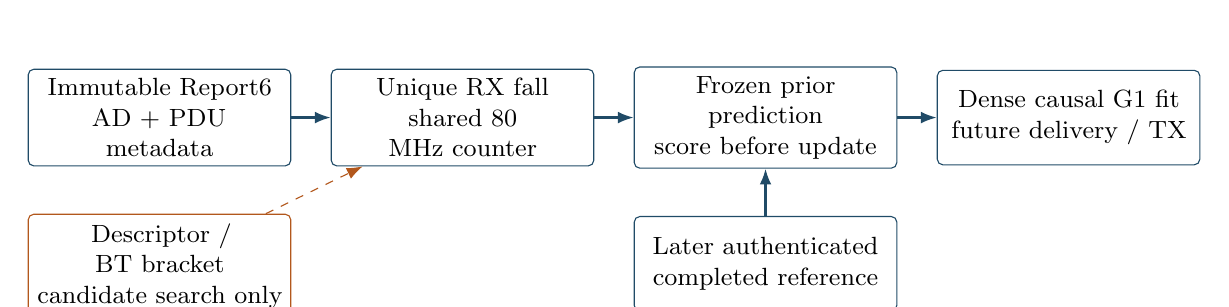
\begin{tikzpicture}[node distance=6mm and 5mm,box/.style={draw=studyblue,rounded corners=2pt,align=center,font=\small,minimum height=12mm,text width=31mm},arr/.style={-{Latex[length=2mm]},draw=studyblue,thick}]
\node[box] (packet) {Immutable Report6\\AD + PDU metadata};
\node[box,right=of packet] (edge) {Unique RX fall\\shared 80 MHz counter};
\node[box,right=of edge] (score) {Frozen prior prediction\\score before update};
\node[box,right=of score] (fit) {Dense causal G1 fit\\future delivery / TX};
\draw[arr] (packet)--(edge);\draw[arr] (edge)--(score);\draw[arr] (score)--(fit);
\node[box,below=of packet,draw=studyorange] (search) {Descriptor / BT bracket\\candidate search only};
\node[box,below=of score] (ref) {Later authenticated\\completed reference};
\draw[dashed,draw=studyorange,-{Latex[length=2mm]}] (search)--(edge);\draw[arr] (ref)--(score);
\end{tikzpicture}
\caption{Implemented event/reference flow. The coarse bracket identifies candidates without supplying receive phase. Original capture prediction is retained before later completed truth trains the clock. TX is still estimated.}
\end{figure}

\subsection{One continuing counter; explicit export accounting}
One boot-owned extended counter now serves RX, CURRENT, reference availability/completion, Bluetooth-clock mapping and TX estimates. There is no mixed-counter fallback. Nominal 32-bit wrap is 53.6870912 s, half-wrap 26.8435456 s. Stale events, counter restart, bad rate/progress or incarnation mismatch withdraw timing authority. The existing dense 64-point causal discipline and source-expiry behavior remain; a later reference cannot improve the prediction previously frozen at capture.

The witness receives the relay while retaining its existing $+10{,}543\ns$ normalization. Eligibility requires enabled diagnosis, valid map, reference seen/fix/PPS, frozen exact scope and reason zero. Invalid numeric phases remain exported. In the completed window, captured dropped/expired/truncated/refused/write/frame-error deltas were all zero. The audit retained 403 N30 raw-CRC and 1565 witness CRC frames; 763 not-found responses were empty polls. RAM overwrite count rose 64 to 728 as ring retention advanced; with zero cursor gaps this is not missing exported data. A capture latch is not an event FIFO, so clean callback/export sequences alone cannot prove every physical transition survived before interrupt service.
\newpage

\section{Controlled marker comparison and internal quality}\label{sec:controlled}
\subsection{Discovery favored RX fall, without qualifying the endpoint}
The first eight deterministic windows retained 16 edges and eight clean windows. Seven had exact common packets and one did not. No late invalidation or audit missing record was observed; maximum audit-query gap was 0.634 s. On the seven pairs, an in-sample affine raw-counter comparison gave 55.523 ns RMS for RX fall, 42.738 $\mu$s for RX rise and 169.588 ns for legacy descriptors. Counter origin and drift were fitted. Those discovery residuals selected a hypothesis; they are not held-out causal output accuracy.

The independent Nordic audit joins the same complete AD using wire peer/root boots and epochs, train, publication, event, channel and AD CRC, with actual path identities checked separately. Device-local capture epochs are not compared as if shared. Correction-completion records and S3-trained projected nanoseconds do not substitute for raw radio capture. CRC proves byte identity, not authentication; the Nordic RX audit producer follows authenticated decoding.

All paired discovery packets used the same PHY/PDU/header class. They cannot establish the fall's RF END/ADDRESS meaning or behavior under other lengths, empty windows and failed packets. The fine-specific composite was calibrated anew rather than inheriting the legacy path correction.

\subsection{A prespecified causal comparison improved but missed 100 ns}
The next 128 deterministic selections were split into 64 training and 64 held-out opportunities. Across all selections, 127 had unique marker windows, 122 exact common packets and six unpaired windows; one training marker window was ambiguous. The held-out population had 62 scored pairs, two unpaired and zero unrecorded. No replacement or residual-based cut selected a better population.

\begin{table}[ht]\centering\small
\caption{Matched held-out scores from the prespecified sparse last-eight-prior/minimum-four affine comparator. This is distinct from production dense G1 and downstream PPS.}
\begin{tabular}{L{73mm}rr}\toprule
Property & Fine marker & Matched legacy\\\midrule
Held-out scored / unpaired&\multicolumn{2}{c}{62 / 2; zero unrecorded}\\
Causal mean (ns)&$-6.807$&$-7.247$\\
Uncentered RMS (ns)&171.004&259.324\\
Maximum absolute residual (ns)&452.233&642.966\\
Paired span / local wraps&\multicolumn{2}{c}{332.998 s / 6}\\
Audit missing / late invalidated&\multicolumn{2}{c}{0 / 0}\\\bottomrule\end{tabular}\end{table}

Conditional RMS improved 34.1\% for matched held-out scores, while remaining above 100 ns. Reference-availability ordering was fixed; no later truth entered a prior prediction. Incomplete channel coverage and the separate sparse estimator limit generalization. The result supports a causal marker improvement on this population, not a 171 ns bound for production G1 or actual output.

\subsection{Internal precision and a repaired resource fault}
The completed N32 research session records three finite internal causal Sync RMS readings of 49 ns among 311 finite readings in 313 snapshots, with steady readings around 53 ns. These are capture-time pre-update prediction-quality values, not downstream PPS error. The 313 normal status snapshots include acquisition and are exported separately; their rolling RMS is neither a whole-run aggregate nor continuous-lock proof.

An earlier low-internal-RMS image later encountered HCI 0x07 Memory Capacity Exceeded during advertising-data update. The tested revision removes unused mutually exclusive WINDOW storage (about 7488 allocated DRAM bytes) and repairs maintenance clock-shutdown ordering. The completed cohort retained one counter incarnation with no reported counter fault, late invalidation or timeout, and sampled healthy status to at least 761.056 s. This is finite post-repair evidence, not long-term reliability certification.
\newpage

\section{Observed bottlenecks and comparison limits}\label{sec:bottlenecks}
\subsection{The short prefix did not contain the later large errors}
\begin{figure}[ht]\centering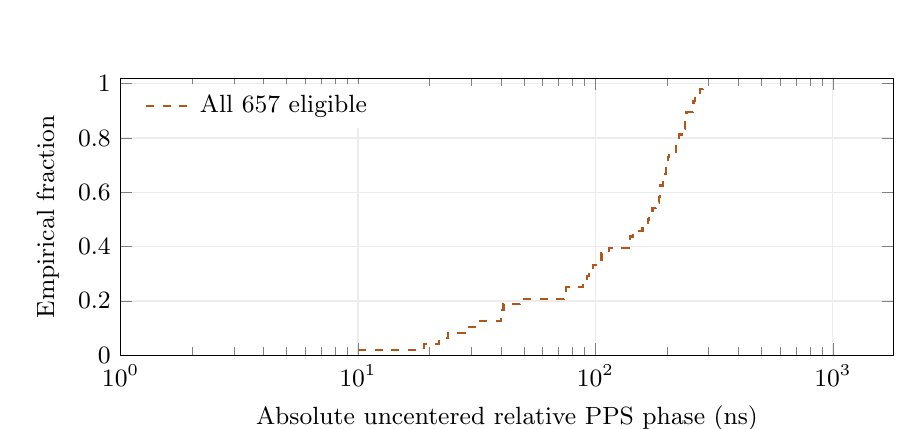
\begin{tikzpicture}
\begin{axis}[width=.94\linewidth,height=51mm,xmode=log,xmin=1,xmax=1800,ymin=0,ymax=1.02,xlabel={Absolute uncentered relative PPS phase (ns)},ylabel={Empirical fraction},grid=major,grid style={gray!15},tick label style={font=\small},label style={font=\small},legend style={font=\small,at={(.02,.98)},anchor=north west,draw=none,fill=white}]
\addplot[studyblue,thick,const plot] coordinates {\FineEcdf};\addlegendentry{All 657 eligible}
\addplot[studyorange,dashed,thick,const plot] coordinates {\SubsetEcdf};\addlegendentry{First 48 subset}
\end{axis}\end{tikzpicture}
\caption{Actual uncentered residual distributions. The full curve reaches 1591 ns; the first 48 are a subset, not an independent trial. Zero is represented at the left logarithmic plotting boundary. Three invalid rows are excluded from residual curves and counted separately.}
\end{figure}

The short subset's 89.089 ns centered spread did not bound the full cohort's 127.842 ns spread. The largest excursions appeared after the first two minutes and again near seven minutes. Neither the earlier 77.382 ns training spread nor a later mean correction qualifies a sub-100 ns result. There is no evidence here that a constant offset removes the mechanism behind the four tails.

\subsection{TX remains a software estimate with measured bracket width}
The relay advertises a reference derived from a programmed scheduling point, not an actual RF TX latch. The implementation reads four Bluetooth-clock brackets, selects the narrowest, uses its midpoint and projects the programmed point through a frozen map. Retained proof brackets span approximately 7.9--9.25 $\mu$s; the controller field retains 500 ns quantization. One continuing local counter removes a mixed-domain phase bridge, but does not turn that software estimate into physical TX time.

Nominal ADDRESS-convention conversion is 40 $\mu$s; integer map projection can yield 39,999 or 40,000 ns. Proof pairs verify that nominal and residual terms sum to the installed total. They do not bound scheduling, detector, RF or propagation error. Bracket midpoint latency/asymmetry and quantization are plausible contributors to boot bias or tails, not a proven sole cause. Counter origins from different boots are not comparable phase measurements.

\subsection{Nordic history retains its own denominators}
Nordic nRF52840 exposes RADIO ADDRESS, TIMER capture and PPI event routing; its nominal 16 MHz grid is 62.5 ns \cite{nordic}. That defined hardware event is an endpoint advantage over the S3's empirical receive-active fall and estimated TX. Detector and antenna delay still require calibration; nominal tick size is not output accuracy.

The preserved V14 one-relay population has 602 nominal opportunities: 436 reference-valid causal, 65 invalid, three expired and 98 unobserved. Conditional mean is $-18.417\ns$, RMS 62.504 ns, standard deviation 59.729 ns and maximum 191 ns, at 72.425\% nominal eligible coverage. Its 501-sample all-causal set including invalid references has 3.929 ms RMS and 19.753 ms maximum; the largest witness gap is 59.017 s \cite{v14}. The new S3 population has greater finite eligible coverage and larger conditional error. Different source paths, dates, estimators and validity patterns preclude a controlled SoC ranking. The older Nordic result is context, not a target already attained by the S3.
\newpage

\section{Concrete remaining improvements}\label{sec:improvements}
The measured priorities are to replace estimated TX, establish the RX reference convention's physical delay, investigate tails and test transfer on a fresh population. The existing common counter is retained throughout. The completed full-window statistics, rather than a favorable prefix or training spread, define the work still required. No proposed mechanism is counted as a result.

\subsection{Verify actual TX and its association}
Freeze the exact selected advertising bank and programmed-map snapshot independently of bulk logging. Correlate the actual transmitted packet with a local event latch and an independent Nordic raw ADDRESS record, retaining no-match, multiple-match and late cases. GPIO5 TX-active is only a candidate signal. A qualified TX timestamp requires both exact packet identity and an independently established RF endpoint/delay. The existing nine-pair proof establishes advertised arithmetic alone.

A new latch must live in the same counter domain as RX, CURRENT, completion and availability. It must preserve source expiry, counter-fault withdrawal and actual reference-availability ordering. Demonstrating narrower software brackets without measuring the event would leave the current physical TX uncertainty unresolved.

\subsection{Resolve RX delay and investigate the tails}
Repeat RX rise/fall correlation with independent raw events while varying real PHY/PDU/header lengths, and include empty, failed and unrelated-traffic windows. The present supported class alone cannot separate RF END, gate delay and timeout behavior. An affine intercept absorbs counter origin and fixed path delay; a small fitted residual therefore cannot calibrate phase. Retain the empirical convention and UNKNOWN endpoint where alternatives remain indistinguishable.

Investigate the four retained large excursions using immutable packet, map-activation and counter-health records. Test candidate causes prospectively, rather than removing the affected samples or renaming them invalid after observing their error. A fixed offset may reduce bias, but the observed mean-only floor is already above 100 ns. Any change intended to reduce variance or tails requires new held-out output observations with fixed scoring and coverage rules.

\begin{table}[ht]\centering\small
\caption{Next measurable decisions. These are uncompleted validation tasks, not predicted improvements.}
\begin{tabular}{L{33mm}L{112mm}}\toprule
Change or check & Required observation before claiming success\\\midrule
Actual TX capture &Same transmitted AD, native local latch and independent RF-correlated endpoint; all unmatched/ambiguous cases retained.\\
RX endpoint/delay &Varied PHY/length and failed/empty controls; delay variation and independent timing uncertainty stated, not absorbed into an unexplained constant.\\
Clock-map delay &Event capture, map activation and completion availability share the continuing counter; no later reference trains an earlier score.\\
Tail reduction &Fresh fixed-population output comparison including every eligible extreme, invalid record and missing opportunity; no evaluation-set offset fit or residual cut.\\
Sub-100 ns / 62.5 ns &Treat these as distinct delivered-relative-PPS RMS targets with maximum and coverage reported. A timer grid or internal fit does not pass either target.\\
Broader transfer &Additional boots/boards on a frozen profile, with identity/scope and advertised arithmetic established before scoring. The completed N31 short check retained a nonzero mean; keep unavailable attempts explicit.\\\bottomrule\end{tabular}\end{table}

The final 51,016 ns N31 transfer retained a $+115.167\ns$ mean and 150.954 ns RMS. Its 64 records include 16 invalid and no software sequence gaps. No further experiment or second long run is included beyond this final short transfer. A quick transfer check can expose a large board/boot bias; it cannot establish long-term tails or calibrated physical output. Subsequent improvements must be judged on a new population after the mechanism changes.
\newpage

\section{Reproduction and practical limits}\label{sec:limits}
\subsection{What the reported error measures}
The witness projects its delivered BLE map at a locally captured PPS and wraps the signed fractional phase into $[-0.5,0.5)$ s. PPS-to-UTC association is zero and absolute-error output unavailable. Shared upstream errors can cancel; fixed receiver, detector, normalization and propagation biases may remain. No N30 electrical PPS output or calibrated absolute UTC error is measured. One-second sampling misses subsecond excursions.

For eligible phases we report signed mean, uncentered RMS, population standard deviation, nearest-rank absolute quantiles and absolute maximum. Invalid records retain their flags and numeric values but do not enter those statistics. No demeaning, detrending, residual cut or independent-sample confidence interval is used. Sequence order, duplicate conflicts and the post-window fence audit native-window export; callback completeness cannot establish RF-latch completeness.

One finite source/path and supported packet class cannot qualify other boots, boards, RF environments, temperatures, distances, lengths or PHYs. Sampled status and a finite healthy session do not prove uninterrupted lock or long-term service. The sparse comparison, dense internal quality, downstream PPS and historical Nordic population have different estimators and denominators and remain separate.

\subsection{Public reconstruction and edition identity}
The selected supplement \cite{supplement} retains all 51 fine-calibration, 660 fixed-window and 64 N31-transfer records, including 22 invalid rows across those populations. It also retains 313 sampled normal snapshots and provenance-bound association/comparison summaries. Private hardware/root identities are reduced to scope-validity flags; enrollment, raw logs, firmware images, absolute epochs, USB identifiers and private paths are excluded. Hashes establish byte identity, not accuracy.

Run \code{python3 tools/verify\_s3\_fine\_paper.py} from a public checkout. Standard-library Python recomputes eligibility, residuals, tails, quantiles, minute blocks, the first-48 subset, offset arithmetic and denominators, then checks selected source/PDF/manifest hashes. No hardware, credentials or sibling private checkout is required. Discovery/sparse summaries are selected aggregates; the public export cannot reconstruct their original RF extraction. The previous reviewed edition and manifest remain unchanged in Git; its original verifier runs at the recorded historical revision. This draft's receipt records the matching source/PDF, compiler and all-page render review.

The hard result is a complete finite window with 166.590 ns RMS and a 1591 ns maximum, alongside a separate matched causal marker gain. The measured output targets remain unmet. The implemented common counter and exact association are useful foundations; verified TX, resolved RX delay, prospective tail reduction and fresh transfer evidence remain the next concrete work.

\begin{thebibliography}{5}\small\setlength{\itemsep}{2pt}
\bibitem{mcpwm} Espressif, \emph{ESP-IDF v5.5.5 Programming Guide: MCPWM, ESP32-S3}, capture timer resolution and event capture. \url{https://docs.espressif.com/projects/esp-idf/en/v5.5.5/esp32s3/api-reference/peripherals/mcpwm.html}.
\bibitem{nordic} Nordic Semiconductor, \emph{nRF52840 Product Specification}, RADIO ADDRESS, PPI and TIMER capture. \url{https://docs.nordicsemi.com/r/bundle/ps_nrf52840/page/radio.html}; \url{https://docs.nordicsemi.com/r/bundle/ps_nrf52840/page/timer.html}.
\bibitem{v14} J. Yantis, \emph{Passive Precision Time over BLE: V14 Boundary Clocks, Causal Timestamping, and Prospective One-Relay Validation}, research draft, 12 October 2026. Historical evidence: \url{https://github.com/yantisj2/PToB/tree/main/evidence/v14/2026-10-12}.
\bibitem{previous} J. Yantis, \emph{Precision Bluetooth Timing on ESP32-S3}, first reviewed draft, 22 October 2026. Immutable manifest \path{papers/editions/s3-timing-2026-10-22.json}; original evidence \path{evidence/s3/2026-10-22}. Source/PDF preserved at the revision recorded in the follow-up receipt.
\bibitem{supplement} J. Yantis, \emph{ESP32-S3 empirical fine-capture follow-up}, selected derived evidence, 22 October 2026. \path{evidence/s3/2026-10-22-fine}; \path{papers/editions/s3-timing-2026-10-22-fine.json}. Original paper, figures and datasets CC BY 4.0; code and ordinary documentation MIT. Research draft, not submitted or promoted.
\end{thebibliography}
\end{document}
